\section{Analyse des conditions optimales du réacteur de synthèse d'ammoniac}

Jusqu'ici nous avons considéré la dernière étape du procédé - la synthèse d'ammoniac -
comme une bo\^ite noire. Nous allons maintenant déterminer quelles sont les conditions 
optimales de température et de pression pour ce réacteur. 
Avant de commencer, il nous semble important de rappeler le principe 
de \textsc{Le Ch\^atelier} : \enquote{Si l'on tend à modifier les conditions d'un système en équilibre, 
il réagit de façon à s'opposer, en partie, aux changements qu'on lui impose, 
jusqu'à l'établissement d'un nouvel équilibre.}. \cite{chatelier}

La réaction de synthèse de l'ammoniac est la suivante
\[\ce{N2_{(g)} + 3H2_{(g)} <=> 2NH3_{(g)} } \]
Nous allons analyser dans les lignes qui suivent les effets de la température, de la pression ainsi que
de la présence d'un catalyseur sur cette réaction. Nous verrons également les limites qui nous sont
imposées par la physique des matériaux utilisés. 

\subsection{Pression}

On voit tout de suite que le nombre de moles de gaz de réactifs est supérieur 
au nombre de moles de gaz des produits, 
plus précisément $n_{g}\text{(réactifs)} = 2 \cdot n_{g}\text{(produits)}$.

Par la loi des gaz parfait, on sait que la pression est directement proportionnelle 
au nombre de moles de gaz. Le principe énoncé ci-dessus
nous permet de dire qu'une \emph{augmentation} de la pression du réacteur ($p_{\text{total}}$),
favorisera le sens de la diminution du nombre de moles de gaz, 
et dans notre cas, favorisera la production de \ce{NH3}.

\[
K = \frac{p_{eq,\ce{NH3}}^2}{p_{eq,\ce{H2}}^3 \cdot p_{eq,\ce{N2}} \cdot p_{\text{total}}^2}
\]
\subsection{Température}

La réaction de synthèse est une réaction fortement exothermique 
(à $700\si{\kelvin}$, $\Delta_r H^{\circ} = -52.6\si{\kilo\joule}$).
Pour favoriser la réaction dans le sens de production des produits,
il faut donc faire une \emph{diminution} de la température.

\[
K = \exp{\left( \frac{- \Delta_r H^{\circ} + T \, \Delta_r S^{\circ}}{R T}\right)}
\]

\subsection{Limite sur la température imposée par le catalyseur}

Après quelques recherches \cite{catalyseur}, 
nous avons découvert que les catalyseurs utilisés
pour la production d'ammoniac en milieu industriel 
contenaient principalement du fer (type \ce{Fe3O4}). 

Pour une usine produisant des quantités de \ce{NH3} similaire à la notre (~$1500$ tonnes/jour), 
une quantité de $100\si{\tonne}$ de catalyseur a une durée de vie d'environ $10$ ans. 
Cependant le catalyseur ne se comporte pas de la m\^eme manière à toutes les températures,
et il s'avère que le catalyseur n'est pas efficace à basse température. 

La réaction risque de devenir trop \emph{lente} pour que le système puisse
atteindre l'équilibre, nous gardons donc la température de $750\si{\kelvin}$
pour la suite de nos calculs.

\subsection{Limite sur la pression imposée par les matériaux du réacteur}

Comme dit auparavant, une haute pression va de paire avec une plus grande production d'ammoniac.
Cependant, le cout pour construire une installation est proportionnel 
à la pression qu'elle pourra supporter. 
De plus, il est également couteux de maintenir une haute pression. 
Il y a donc une pression à partir de laquelle les couts demandés 
par le processus ne sont pas justifiés par rapport aux bénéfices. 

C'est l'aspect \emph{économique} qui est limitant ici et il faut à nouveau trouver un compromis.
Nous avons jugé qu'il est convenable de garder la pression proposée de $270\si{\bar}$ 
pour la suite de nos calculs.

\subsection{Conclusion}

Nous finissons cette première partie de la t\^ache 2
avec les graphes~\ref{fig:efficienceSnoPurge} et~\ref{fig:efficienceCnoPurge}. 
Ceux-ci modélisent le rendement de la réaction en fonction des 
deux paramètres étudiés $p$ et $T$.
On remarque tout de suite que la variation de pression a très peu
d'importance sur le rendement et que c'est principalement
la température qui va déterminer l'efficacité du réacteur.

Le rendement dans ce cas-ci est défini comme 
\[ \eta = \frac{n_{\ce{NH3},\text{équilibre}}}{n_{\ce{NH3},\text{réaction complète}}} \]

\begin{figure}
	\centering
	\begin{subfigure}[b]{1\textwidth}
		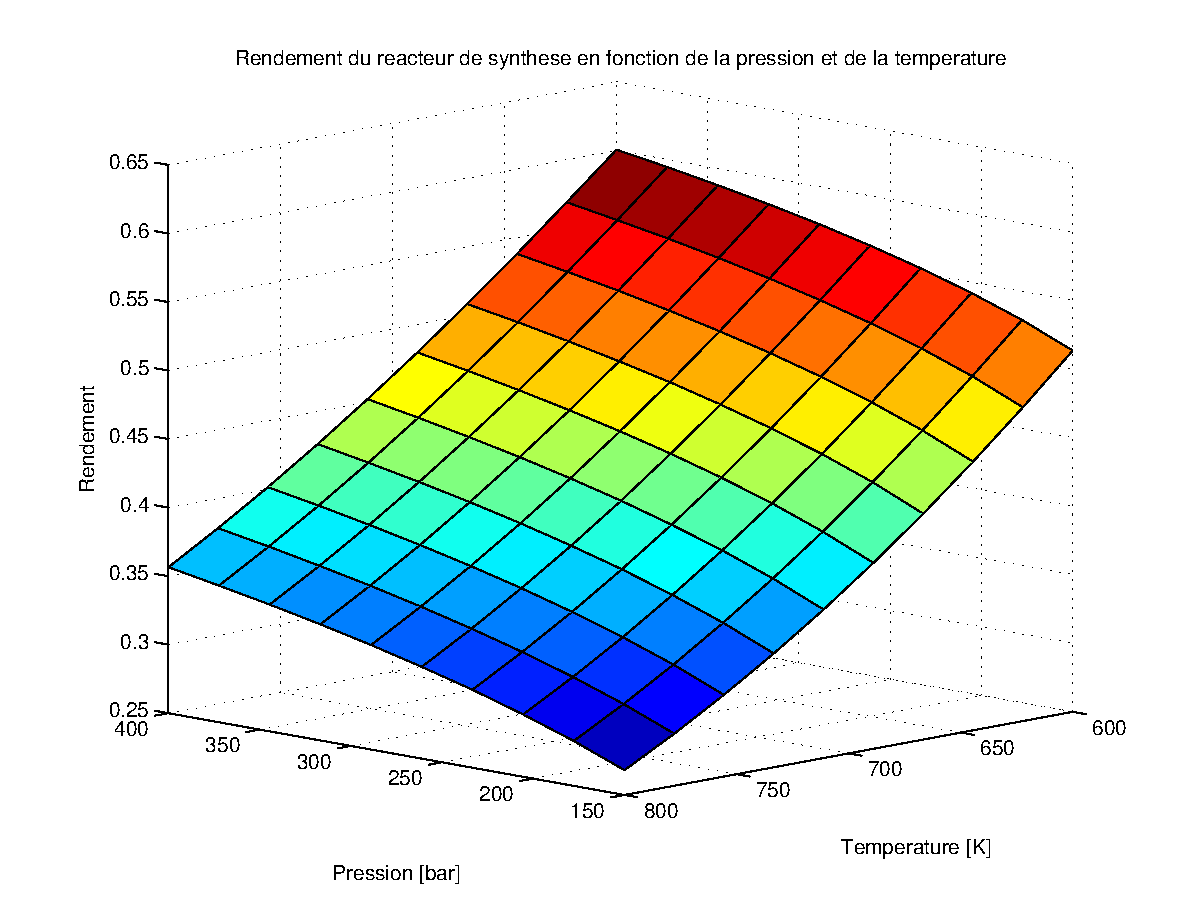
\includegraphics[scale=0.7]{../tache2/img/efficienceSyntheseSnoPurge.eps}
		\caption{Plot 3D.}
		\label{fig:efficienceSnoPurge}
	\end{subfigure}
	\begin{subfigure}[b]{0.8\textwidth}
		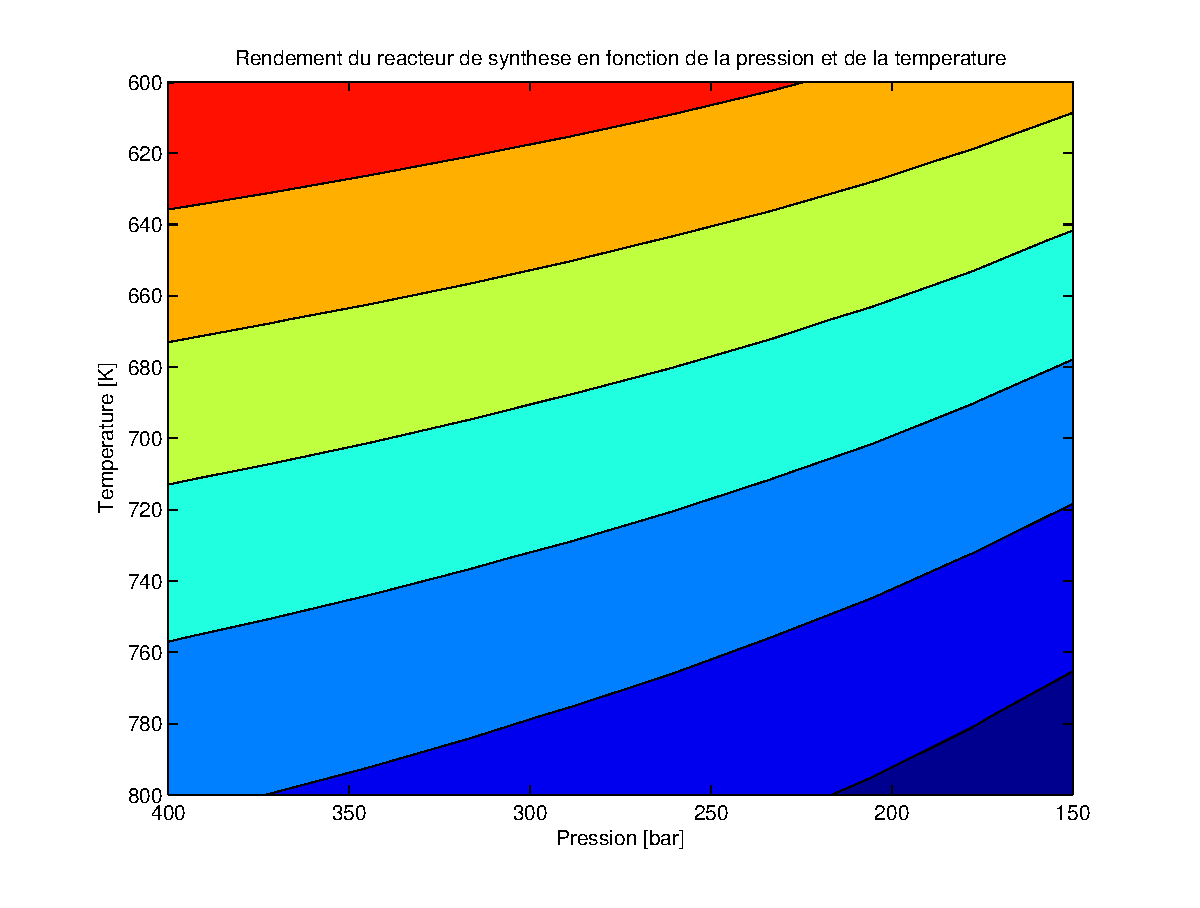
\includegraphics[scale=0.6]{../tache2/img/efficienceSyntheseCnoPurge.eps}
		\caption{Courbes de niveau associés au plot 3D.}
		\label{fig:efficienceCnoPurge}
	\end{subfigure} \\
	\caption{Efficacité du réacteur de synthèse en fonction de la température.
		Le rendement est ici défini comme le rapport $n_{\ce{NH3},\text{équilibre}}/
		n_{\ce{NH3},\text{réaction complète}}$.}
\end{figure}


\section{Modélisation par \textsc{Aspen Plus}}
\subsection{Démarrage}

Lors de la première tâche, nous analysions l'installation dans son ensemble, 
mais de manière excessivement simplifiée. 
Dans cette section, nous nous concentrerons sur l'explicitation de la dernière étape 
pour ensuite la simuler sur le logiciel \textsc{Aspen Plus}. 
Nous ne désirons plus la considérer comme une boîte noire, et l'avons donc découpée 
en un certain nombre de processus intermédiaires. 

Le gaz entrant, composé d'\ce{N2}, d'\ce{H2} et d'\ce{Ar}, passe par un réchauffeur 
et par un compresseur pour atteindre respectivement la température et la pression voulue. 
Il va ensuite dans le réacteur où se déroule la réaction.
Le produit est refroidi dans une installation prévue à cette effet, 
pour arriver enfin dans un séparateur où on extrait l'ammoniac.

Il semblait intéressant de créer un circuit de recyclage pour réutiliser 
le mélange de \ce{N2} et de \ce{H2} issus du processus (la réaction n'est pas complète 
et il reste donc des réactifs). Malheureusement, il y existe également de l'argon 
qu'on ne peut séparer du reste. En effet, sa température d'ébullition est bien trop 
proche de celle des autres composés et les moyens à mettre en œuvre en seraient 
très couteux et/ou à faible rendement.

Notre groupe a donc décidé de faire une purge dans le circuit de recyclage afin d'éviter que l'argon ne s'accumule. Il y a donc une fraction minimale à purger. Mais cette purge ne doit pas être trop grande sinon la quantité perdue des réactifs serait conséquente. 
La condition à respecter est donc d'avoir un flux entrant d'argon égal à celui de sortie lorsque la réaction est en "régime", c'est à dire après un nombre conséquent d'itérations.

Le flowsheet de notre installation correspondant à la modélisation 
du réacteur de synthèse sur \textsc{Aspen Plus} 
se trouve dans la figure \ref{fig:flow_aspen}.
Afin d'apporter plus de précision, nous avons également réalisé un petit 
flowsheet de la même partie du procédé qui détaille le parcours des 
différents réactifs et leurs états à travers le processus.
Le diagramme se trouve dans la figure \ref{fig:flow_synthese}.

\begin{figure}[h!]
	\begin{center}
		\includegraphics[scale=0.45,angle=90]{../tache2/img_aspen/flowsheet.jpg}
	\end{center}
	\caption{Flowsheet de la réaction finale sur \textsc{Aspen Plus}.}
	\label{fig:flow_aspen}
\end{figure}

\subsection{Prévisions}

Dans cette sous-section, nous faisons notre propre simulation de la dernière étape, en considérant
le système à l'équilibre. Les flux y sont donc constants. Notre but est ici de calculer 
le rendement du circuit en terme de production d'ammoniac. 
Nous cherchons donc la quantité d'\ce{NH3} réellement produite.
A cette fin, nous fixons la température et la pression dans le réacteur, ainsi que la fraction X
à purger dans le recyclage.
Nous négligeons l'imperfection du séparateur et faisons donc l'hypothèse 
que l'ammoniac sortant est pur, ce qui est bien s\^ur impossible.
Nous nous référerons au flowsheet pour ce qu'il en est des notations et
faisons l'hypothèse que nous connaissons le flux entrant de réactifs.

\begin{figure}[h!]
	\begin{center}
		\input{../tache2/flow_synthese}
	\end{center}
	\caption{Schéma simplifié de l'étape finale.}
	\label{fig:flow_synthese}
\end{figure}

Comme dit précédemment, la purge doit permettre un débit 
de sortie d'argon égal à celui d'entrée dans le système. 
On peut écrire cela sous la forme:

\begin{equation}
\dot{n}_{\ce{Ar},\text{in}} = \dot{n}_{\ce{Ar},\text{purge}} = 
x_{\ce{Ar},\text{purge}} \cdot \dot{n}_{\text{purge}}
\label{eq:bilan_tot_argon}
\end{equation}

Ceci est donc le bilan total d'argon. 
Il est possible de faire d'autres bilans afin de nous donner d'autres relations utiles.

$\bullet$ Bilan molaire à la purge:
\begin{equation}
\dot{n}_{\text{purge}} = X \cdot \dot{n}_{\text{recyclage}}
\label{eq:bilan_mol_purge}
\end{equation}

$\bullet$ Bilan molaire au séparateur:
\begin{equation}
\dot{n}_{\text{out}}=\dot{n}_{\text{recyclage}}+\dot{n}_{\ce{NH3},\text{out}}
\label{eq:bilan_mol_sep}
\end{equation}

%$\bullet$ Bilan d'argon au séparateur:
%\begin{equation}
%x_{Ar,\text{out}} \dot{n}_{\text{out}}=x_{\ce{Ar},\text{recyclage}} \dot{n}_{\text{recyclage}}
%\end{equation}

$\bullet$ Bilan molaire total:

\begin{equation}
	\dot{n}_{in} - 2\xi=\dot{n}_{\ce{NH3},\text{out}} + \dot{n}_{\text{purge}}
	\label{eq:bilan_mol_tot}
\end{equation}

avec $\xi$ étant l'avancement, c'est à dire le nombre de moles de \ce{N2} ayant réagi. 
Cela est résumé dans le tableau \ref{tab:reaction_purge_eq}.
On analyse le débit de moles à l'entrée du réacteur pour les différents composés, 
ainsi qu'à la sortie (on considère que l'équilibre a été atteint). 
Les indices \textit{rec} et \textit{pur} font respectivement référence au recyclage et à la purge. 
On voit tout de suite que le flux des moles d'ammoniac produites est égal à $2 \xi$. Il
nous faut donc par exemple trouver l'avancement pour obtenir sa valeur. Nous pouvons faire
cela en partant de l'équation d'équilibre.

\begin{table}[h!]
	\centering
	\begin{tabular}{c|c|c|c|c}
		$\ce{N2}$ & $\ce{H2}$ & $\ce{Ar}$ & $\ce{NH3}$ & $n_{\text{total}}$ \\
		\hline
		$n_{\ce{N2},\text{in}}$+$n_{\ce{N2},\text{rec-pur}}$ 
		& $n_{\ce{H2},\text{in}}$+$n_{\ce{H2},\text{rec-pur}}$ & 
		$n_{\ce{Ar},\text{in}}$+$n_{\ce{Ar},\text{rec-pur}}$ &
		$0$  & $n_{\text{in}}$+$n_{\text{rec-pur}}$ \\
		$n_{\ce{N2},\text{in}}$+$n_{\ce{N2},\text{rec-pur}}$ - $\xi$ &
		$n_{\ce{H2},\text{in}}$+$n_{\ce{H2},\text{rec-pur}}$ - $3\xi$ & 
		$n_{\ce{Ar},\text{in}}$+$n_{\ce{Ar},\text{rec-pur}}$ & 
		$2 \xi$  & $n_{\text{in}}$+$n_{\text{rec-pur}}$- $2\xi$\\
	\end{tabular}
	\caption{Réaction dans le réacteur.}
	\label{tab:reaction_purge_eq}
\end{table}

La réaction se déroule à une certaine température T et à une pression p. 
Il est facile de calculer $K$ en trouvant $\Delta_r G$ au préalable. 
Nous pouvons faire cela en utilisant notre outil de calcul.

\[
K=\exp{\left(\frac{-\Delta G}{R \cdot T}\right)}\]

L'expression de la constante d'équilibre $K_p$ est également: 

\[
K_p=\frac{{x_{\ce{NH3},\text{out}}}^2}{x_{\ce{N2},\text{out}} \cdot
	{x_{\ce{H2},\text{out}}}^3} \cdot p^{-2} = 
	\frac{{n_{\ce{NH3},\text{out}}}^2}{n_{\ce{N2},\text{out}} \cdot 
	{n_{\ce{H2},\text{out}}}^3}\cdot {n_{\text{total,out}}}^2\cdot p^{-2}
\]
si on utilise la loi des gaz parfaits et plus précisément celle de Dalton. 
On sait aussi que $n_{\ce{H2}}=3\cdot n_{\ce{N2}}$.
En injectant les quantités des composés du tableau~\ref{tab:reaction_purge_eq},
fonctions de $\xi$, on obtient:

\[ 
K = 
\frac{({2\xi})^2}{27 \cdot ({{n_{\ce{N2},\text{in}}}+x_{\ce{N2},\text{rec}}
(n_{\text{rec}}-n_{\text{pur}})-\xi})^4} \cdot
	({n_{\text{in}}+n_{\text{rec}}-n_{\text{pur}}-2\xi})^2 \cdot p^{-2} 
\]

Rappelons que $x_{i,\text{rec}}=x_{i,\text{pur}}$ car la purge n'altère pas la concentration.
Nous appliquons cela pour simplifier l'expression de l'azote venant du circuit
de recyclage.
Nous devons déterminer les 4 inconnues suivantes : $n_{\text{rec}}$, $n_{\text{pur}}$, 
$x_{N2,\text{rec}}$ et $\xi$.
Nous avons donc besoin de trois autres équations reliant ces dernières pour pouvoir 
résoudre un système à solution unique.

Une première est obtenue avec l'équation \ref{eq:bilan_mol_tot} où on remplace $n_{\ce{NH3},out}$ par
$2 \xi$ (voir tableau \ref{tab:reaction_purge_eq}).
\[n_{\text{pur}}=n_{\text{in}} - 4 \xi \]

On trouve une deuxième grâce à l'équation \ref{eq:bilan_mol_purge} 
où on remplace $x_{Ar,\text{purge}}$ 
par $1-x_{\ce{N2},\text{purge}}-x_{\ce{H2},\text{purge}}=1-4\cdot x_{\ce{N2},\text{purge}}$.
\[ \dot{n}_{\ce{Ar},\text{in}}=(1-4\cdot x_{\ce{N2},\text{purge}}) \dot{n}_{\text{purge}} \]

On utilise enfin l'équation \ref{eq:bilan_mol_purge}, 
ce qui nous permet de résoudre le problème! On peut en effet alors
trouver la valeur des inconnues citées plus haut.
Une manière simple de faire cela est d'utiliser les calcul symbolique de \textsc{Matlab}. 
Comme dit précédemment, la quantité réelle d'ammoniac produite est égale à $2 \xi$ 
et nous pouvons calculer le rendement en divisant ce résultat
par la quantité produite prévue dans le cas d'une réaction hypothétiquement parfaite.

Le même cheminement est suivi dans le programme \texttt{equilibriumSimulation} 
disponible dans notre outil de gestion. Ce dernier nous donne le rendement pour un
certain jeu de paramètres. Un autre programme, \texttt{efficiencePlot}, trace un graphe
tri-dimensionnel de ces résultats avec une purge fixée à $5\%$,
variant avec la température et la pression. 
Comme attendu, le rendement augmente toujours avec la pression et diminue
de manière plus conséquente avec la température. 
Les graphes \ref{fig:efficienceS} et \ref{fig:efficienceC} nous montrent cela.
On remarquera aussi un bien meilleur rendement que lors
de la simulation sans purge (voir figure~\ref{fig:efficienceSnoPurge}),
tout en conservant les mêmes variations par rapport à la température 
et la pression (voir figure~\ref{fig:efficienceCnoPurge}).

\begin{figure}
	\centering
	\begin{subfigure}[b]{1\textwidth}
		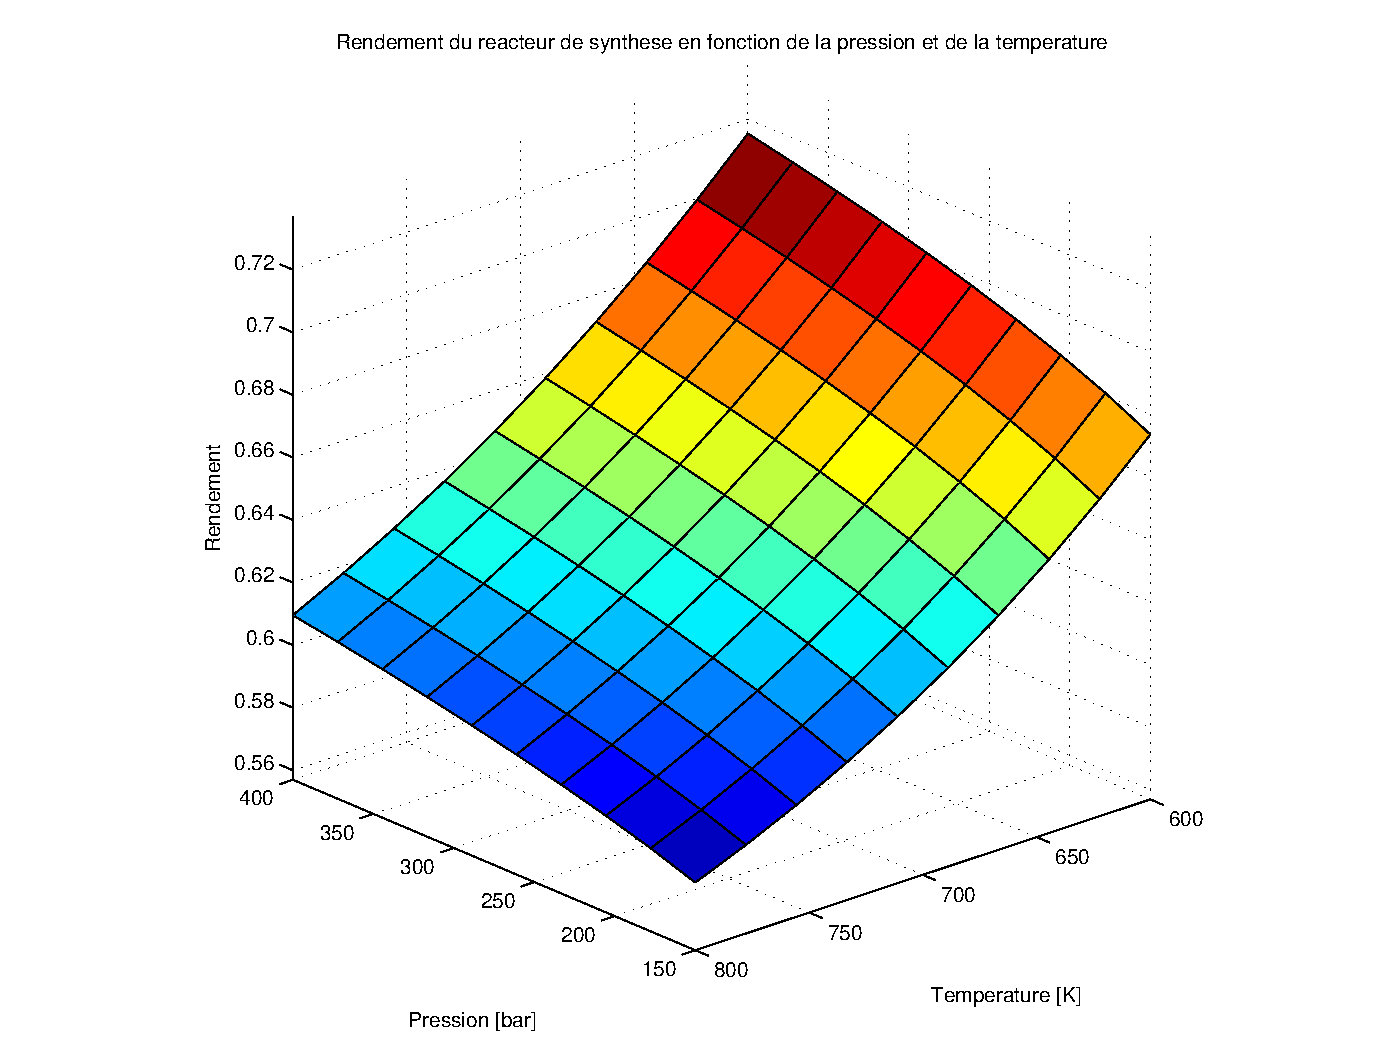
\includegraphics[scale=0.7]{../tache2/img/efficienceSyntheseS.eps}
		\caption{Plot 3D.}
		\label{fig:efficienceS}
	\end{subfigure}
	\begin{subfigure}[b]{0.8\textwidth}
		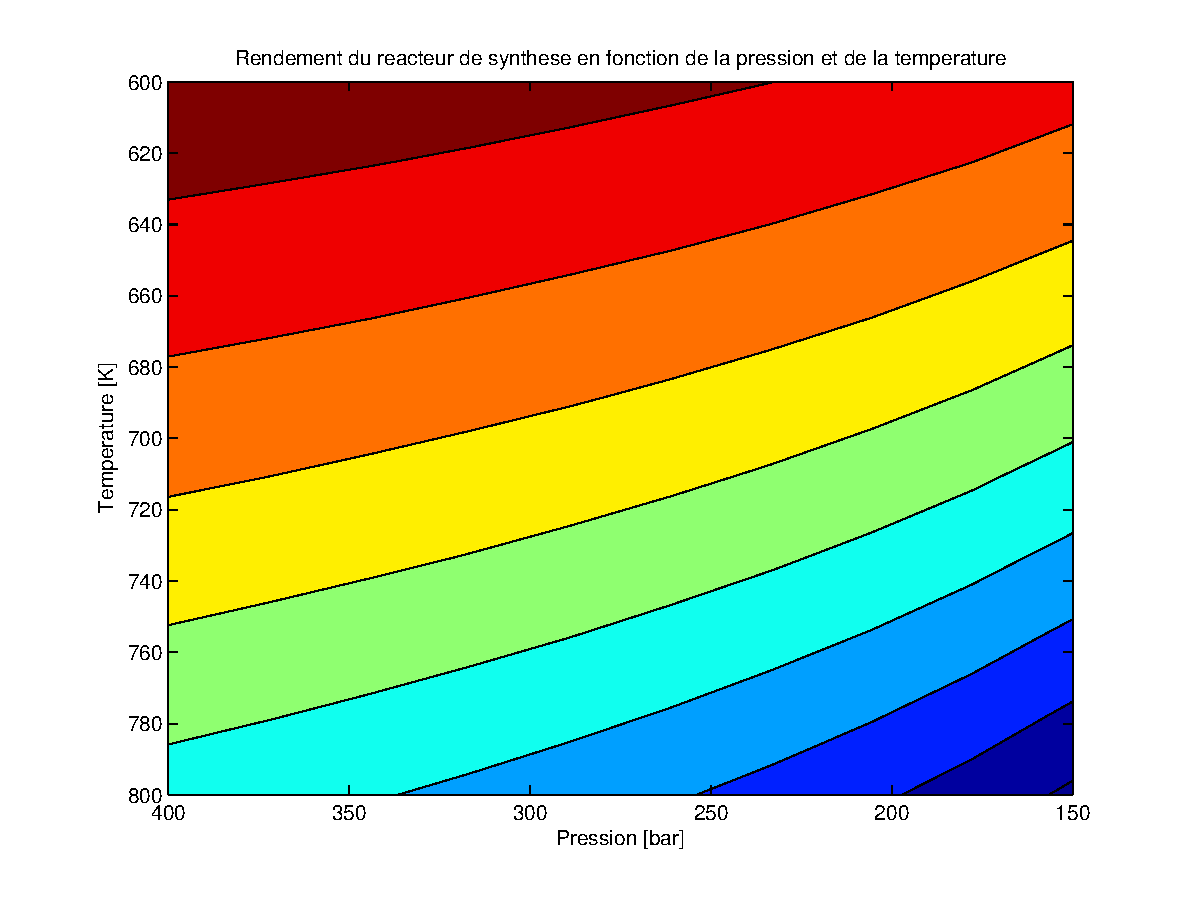
\includegraphics[scale=0.6]{../tache2/img/efficienceSyntheseC.eps}
		\caption{Courbes de niveau associés au plot 3D.}
		\label{fig:efficienceC}
	\end{subfigure} \\
	\caption{Efficacité du réacteur de synthèse en fonction de la température 
		et de la pression en tenant compte d'une perte d'une partie des 
		réactifs (\ce{H2} et \ce{N2}) lors de la purge ($5\%$ dans ce cas),
		nécessaire pour éviter l'accumulation de \ce{Ar}.}
\end{figure}

\subsection{Validation du modèle}

Nous avons alors voulu confirmer nos résultats avec un logiciel 
qui nous permettrait de simuler notre réaction. 
Le logiciel \textsc{Aspen Plus} propose de nombreuses 
modélisations du comportement des fluides, 
plus ou moins fidèles selon les composés et 
les conditions dans lesquelles on les observe. 
Notre recherche s'est limitée aux modèles à haute pression. 

Après en avoir fait l'étude en comparant les bases de données de chacun d'eux, 
nous avons gardé 3 candidats: \texttt{RK-Aspen}, \texttt{PSRK} et \texttt{SRK}. 
Tous trois basés sur les équations de Soave-Redlich-Kwong, 
ils modélisent correctement les gaz légers et non polaires 
comme ceux auxquels nous avons affaire ici. 
Ces modèles sont également les seuls à être capables de faire 
des prédictions correctes à une pression supérieure à $150\si{\bar}$. 
Nous avons donc effectué quelques tests sur chacun des trois 
et nous avons obtenu des résultats assez similaires.
Cependant, le modèle SRK promet de garder sa précision dans des conditions 
quasi critiques, ce qui n'est pas le cas des deux autres. 
La pression dans notre circuit pouvant avoisiner les $270\si{\bar}$, 
c'est ce dernier que nous avons donc choisi pour faire des simulations approfondies.\\
Lors de nos tests, nous avons arbitrairement fixé la température et 
la pression des réactifs entrants respectivement à $25\si{\degreeCelsius}$ et $1\si{\bar}$.

En effet, leurs valeurs exactes nous sont inconnues et n'ont de toute manière 
aucun impact sur le fonctionnement du circuit, grâce à la présence des échangeurs de chaleur 
et du compresseur.

Tout d'abord, nous avons fixé les conditions dans le réacteur à $270\si{\bar}$ 
et $750\si{\kelvin}$. 
Nous avons également choisi de mettre un certain flux de \ce{H2}, \ce{N2}, et d' \ce{Ar} 
pour lesquels nous connaissions le flux théorique correspondant de \ce{NH3} à la sortie,
grâce au tableau de données reçu à la tâche~1. 
Nous avons également fixé le pourcentage du recyclage à purger à $5\%$ pour nos tests.\\

Pour les conditions décrites ci-dessus, 
nous avons obtenu après simulation un flux de \ce{NH3} légèrement inférieur à nos attentes. 
Cela s'explique à nouveau par le fait que pour les résultats attendus, 
nous avions négligé les pertes au niveau du séparateur et considéré la réaction complète.
Par la suite, nous avons essayé de faire varier certains paramètres afin 
de voir si les résultats obtenus étaient en adéquation avec nos prédictions. 
Nous avons commencé par diminuer la température et comme nous l'avions prédit, 
la quantité produite d'ammoniac a augmenté. 
Un test avec une température supérieure à $750\si{\kelvin}$ nous a confirmé cela. 
Nous avons ensuite vérifié que nos attentes concernant la pression étaient respectées. 
Et en effet, lorsque nous avons augmenté la pression, 
la quantité produite de \ce{NH3} a faiblement augmenté.

Pour finir, nous avons fait varier les valeurs du pourcentage de la purge.
Il s'est avéré que notre simulation ne convergeait pas en dessous de $4\%$ 
et nous avions des erreurs.
Nous avons ensuite augmenté le pourcentage 
et observé une diminution de la production de \ce{NH3}. 
Ces résultats sont logiques puisque l'augmentation du pourcentage 
de purge est évidemment la cause de pertes de matières premières. 
La quantité de produits en est donc altérée.

Tous les résultats obtenus lors de nos simulations 
sont disponibles dans l'annexe~\ref{sec:aspen_simulation}.

\subsection{Simulation itérative sur \textsc{Matlab}}

Nous avons choisi de créer une seconde simulation
pour comparer les résultats obtenus ainsi que 
les conditions menant à la convergence.
Son fonctionnement est simple:
elle calcule - pour une série d'itérations - 
les différents flux à la sortie du réacteur 
et dans le recyclage grâce à l'avancement de
la réaction. On utilise ensuite ces informations 
de manière récursive pour connaître le débit de 
réactifs entrants au prochain pas de temps. Si 
la différence entre le flux d'argon actuel et 
de l'itération précédente passe en dessous d'un 
certain seuil, on considère que le système s'est 
stabilisé: il a convergé.

Il se trouve que les résultats de nos deux simulations
sont exactement identiques! Et pour ce qu'il en est
de la simulation sur \textsc{Aspen Plus}, les résultats sont
remarquablement proches malgré les imprécisions du modèle
utilisé, à savoir, que l'installation
est parfaite et que les gaz sont parfaits.

On remarque cependant une divergence marquée lorsque l'on travaille 
avec une haute température. A titre d'illustration, 
la figure \ref{tab:sim} nous donne la comparaison 
de résultats venant des deux simulations:

\begin{table}[h!]
	\centering
	\begin{tabular}{l|c|c}
		Paramètres choisis & $n_{\ce{NH3}}$ - \textsc{Aspen} & $n_{\ce{NH3}}$ - \textsc{Matlab}\\
		\hline
		 T=750K, p=270bar  x=5\% & 942,94mol/s & 937,795mol/s \\

		\hline\hline

		T=500K, p=270bar, x=5\% & 1011,06mol/s & 999,335mol/s \\

		\hline\hline

		T=750K, p=220bar, x=5\% & 929,115mol/s & 931,36mol/s \\
		
		\hline\hline
		
		T=750K, p=270bar, x=10\% & 883,132mol/s & 869,733mol/s \\
		\hline
	\end{tabular}
	\caption{Comparaison des simulations pour $m_{\ce{NH3}, \text{théorique}}=1500$t/jour.}
	\label{tab:sim}
\end{table}

\section{Résultats des simulations sur \textsc{Aspen Plus}}
\label{sec:aspen_simulation}

Nous regroupons dans les figures~\ref{fig:RK-ASPEN} à~\ref{fig:SRK,750,270,1}
tous les résultats produits par nos simulations réalisées sur \textsc{Aspen Plus}. 
Pour chacune d'elles, nous précisons le modèle utilisé,
les conditions de température et de pression dans le réacteur 
et la fraction purgée du recyclage. 
On accorde en particulier de l'attention aux résultats 
concernant les deux flux suivants: \textsc{nh3,out} et \textsc{purge}.

\graphicspath{{./img_aspen/}}

\begin{figure}[h!]
	\begin{center}
		\includegraphics[scale=0.5]{RK-ASPEN.png}
	\end{center}
	\caption{Modèle \texttt{RK-ASPEN}, $750\si{\kelvin}$, $270\si{\bar}$, 5\%}
	\label{fig:RK-ASPEN}
\end{figure}

\begin{figure}[h!]
	\begin{center}
		\includegraphics[scale=0.5]{PSRK.png}
	\end{center}
	\caption{Modèle \texttt{PSRK}, $750\si{\kelvin}$, $270\si{\bar}$, 5\%}
	\label{fig:PSRK}
\end{figure}

\begin{figure}[h!]
	\begin{center}
		\includegraphics[scale=0.5]{SRK,750,270,5.png}
	\end{center}
	\caption{Modèle \texttt{SRK}, $750\si{\kelvin}$, $270\si{\bar}$, 5\%}
	\label{fig:SRK,750,270,0.05}
\end{figure}

\begin{figure}[h!]
	\begin{center}
		\includegraphics[scale=0.5]{SRK,500,270.png}
	\end{center}
	\caption{Modèle \texttt{SRK}, $500\si{\kelvin}$, $270\si{\bar}$, 5\%}
	\label{fig:SRK,500,270,0.05}
\end{figure}

\begin{figure}[h!]
	\begin{center}
		\includegraphics[scale=0.5]{SRK,1000,270.png}
	\end{center}
	\caption{Modèle \texttt{SRK}, $1000\si{\kelvin}$, $270\si{\bar}$, 5\%}
	\label{fig:SRK,1000,270,0.05}
\end{figure}

\begin{figure}[h!]
	\begin{center}
		\includegraphics[scale=0.5]{SRK,750,220.png}
	\end{center}
	\caption{Modèle \texttt{SRK}, $750\si{\kelvin}$, $220\si{\bar}$, 5\%}
	\label{fig:SRK,750,220,0.05}
\end{figure}

\begin{figure}[h!]
	\begin{center}
		\includegraphics[scale=0.5]{SRK,750,300.png}
	\end{center}
	\caption{Modèle \texttt{SRK}, $750\si{\kelvin}$, $300\si{\bar}$, 5\%}
	\label{fig:SRK,750,300,0.05}
\end{figure}

\begin{figure}[h!]
	\begin{center}
		\includegraphics[scale=0.5]{SRK,750,270,4.png}
	\end{center}
	\caption{Modèle \texttt{SRK}, $750\si{\kelvin}$, $270\si{\bar}$, 4\%}
	\label{fig:SRK,750,270,0.04}
\end{figure}

\begin{figure}[h!]
	\begin{center}
		\includegraphics[scale=0.5]{SRK,750,270,10.png}
	\end{center}
	\caption{Modèle \texttt{SRK}, $750\si{\kelvin}$, $270\si{\bar}$, 10\%}
	\label{fig:SRK,750,270,0.1}
\end{figure}

\begin{figure}[h!]
	\begin{center}
		\includegraphics[scale=0.5]{SRK,750,270,50.png}
	\end{center}
	\caption{Modèle \texttt{SRK}, $750\si{\kelvin}$, $270\si{\bar}$, 50\%}
	\label{fig:SRK,750,270,0.5}
\end{figure}

\begin{figure}[h!]
	\begin{center}
		\includegraphics[scale=0.5]{SRK,750,270,100.png}
	\end{center}
	\caption{Modèle \texttt{SRK}, $750\si{\kelvin}$, $270\si{\bar}$, 100\%}
	\label{fig:SRK,750,270,1}
\end{figure}


